\author{Emanuele Carraro}

\title{Project report for Bioinformatics course}
\maketitle

\newpage
\tableofcontents

\newpage
\section{Project report}

In the directory you will find the genomic reference sequence of a bacterium
called Lactobacillus casei. The genome is \texttt{3,079,196} bp long.

The aim of the project is the ``resequencing'' of a similar
bacterium that we call lact.sp, using mate pairs reads.

In particular we want to see if lact.sp has genomic structural variations.

We suspect that the lact.sp genome may have small and large deletions,
insertions and inversions, and we want to find where they are.

The mate pairs fastq reads are supplied in two files.
\subsection{Part 1}

\begin{enumerate}
\item Download the reference genome and the zip file with the fastq reads
\item Install BWA on your computer
\item Use BWA to align the illumina reads on the reference genome
\item Install IGV on your computer
\item Process the sam file obtained by the BWA analysis to make a bam file
\item Sort and index the bam file (see unix.pdf)
\item Visualize the coverage and mate pairs on the IGV
\item Manually find and comment any ``anomalous'' pair of mates
\end{enumerate}

\subsection{Part 1 - Answers}
\begin{enumerate}
  \item This part was done in classroom
  \item This part was done in classroom
  \item Enter the following command in the directory with the reads and the
reference genome: \texttt{bwa index Lactobacillus\_casei\_genome.fasta} and
\texttt{bwa mem Lactobacillus\_casei\_genome.fasta lact\_sp.read1.fastq 
lact\_sp.read2.fastq > lact\_sp.sam}
  \item This part was done in classroom
  \item Enter the following command:
\texttt{samtools view -bS lact\_sp.sam > lact.bam}
  \item Enter the following command:
\texttt{samtools sort lact.bam lact\_sorted} and
\texttt{samtools index lact\_sorted.bam}
  \item In figure \ref{fig:coverage_matepairs} there is a screen of IVG
interface with the coverage (\texttt{lact\_sorted.bam.Coverage}) and mate pairs
(\texttt{lact\_sorted.bam})

\begin{figure}[h]
  \centering
  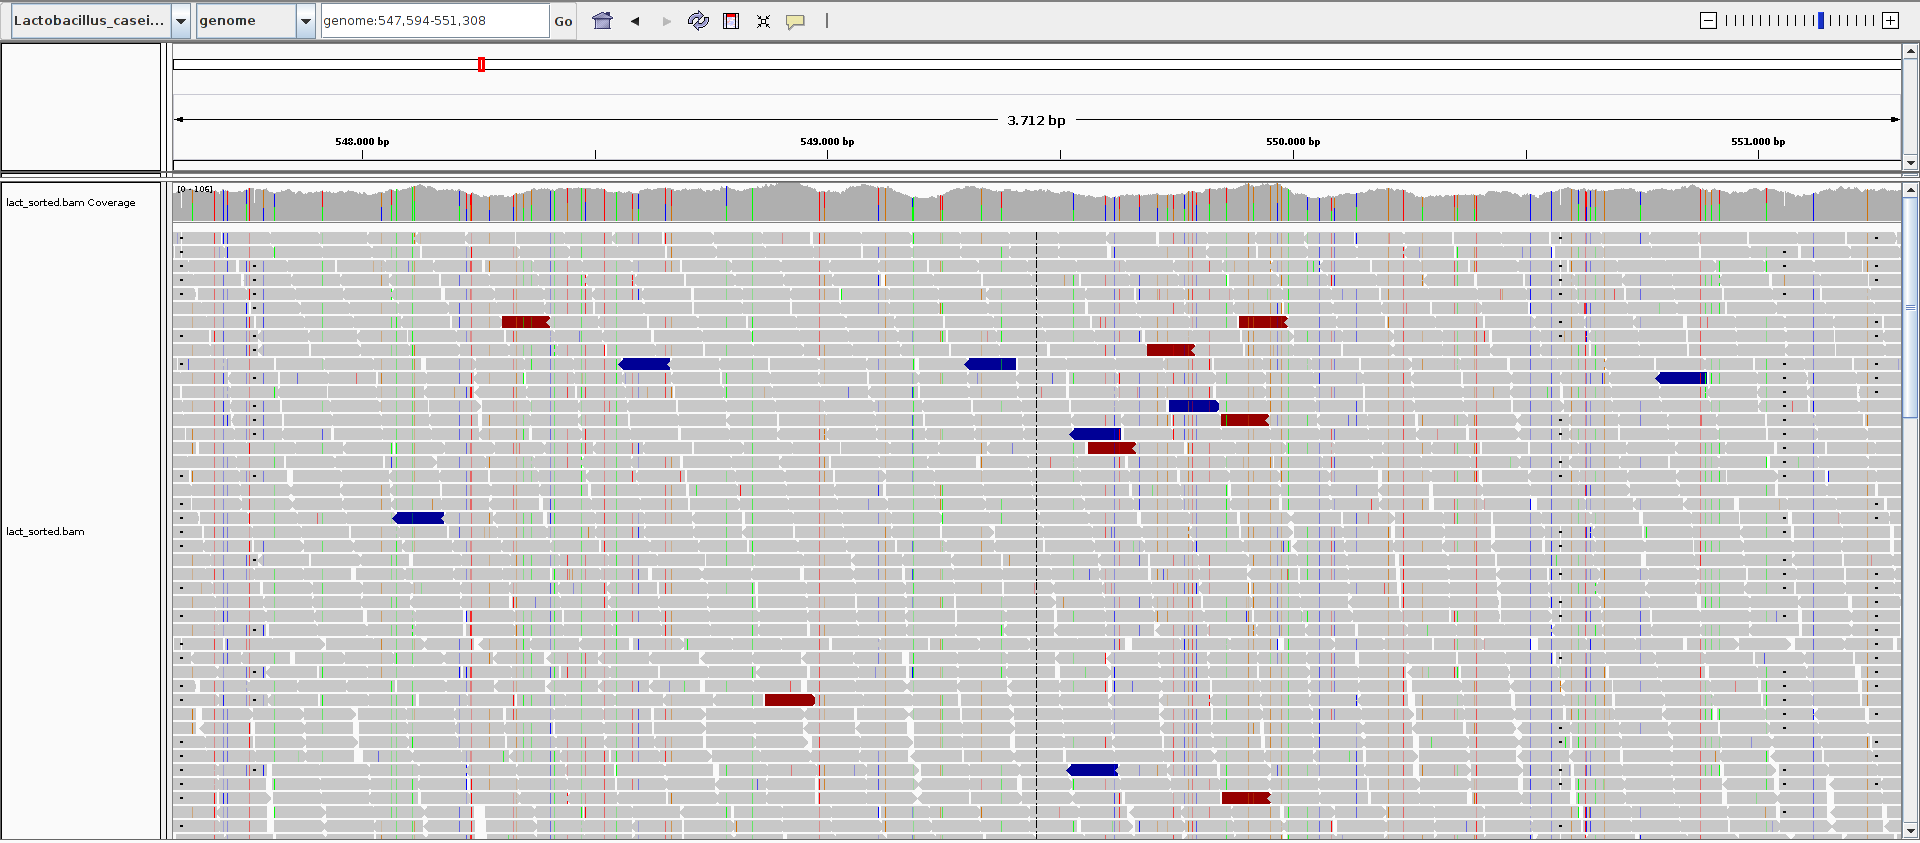
\includegraphics[scale=0.2]{img/coverage_matepairs}
  \caption{Coverage and mate pairs on the IGV}
  \label{fig:coverage_matepairs}
\end{figure}

  \item We can observe that in the figure \ref{fig:pairs} that there is a long
deletion. Reads that are colored red have larger size than expected, 
and therefore indicate possible deletions.

\begin{figure}[h]
  \centering
  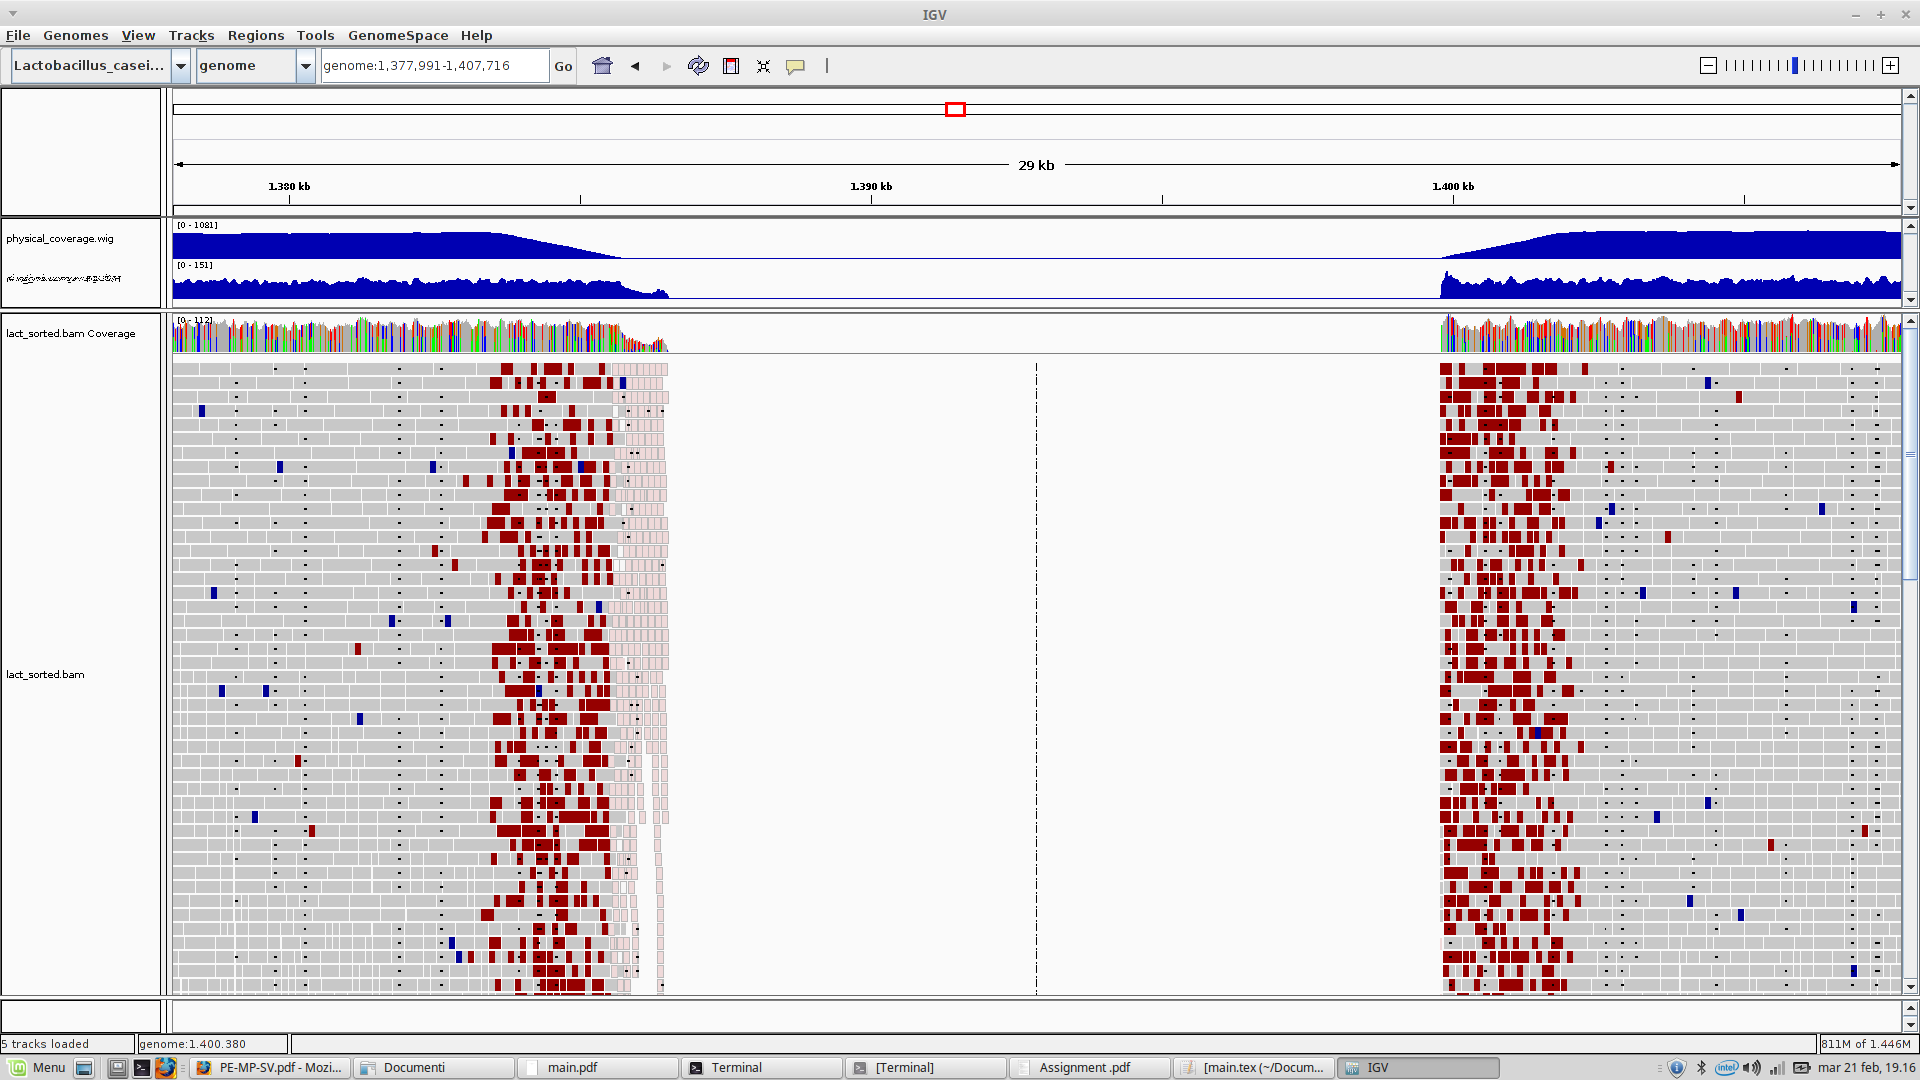
\includegraphics[scale=0.2]{img/pairs}
  \caption{Long deletion}
  \label{fig:pairs}
\end{figure}

Reads that are colored blue have smaller size than expected, and therefore
indicate insertions. We can observe some of them in figure
\ref{fig:pairs2}.

\begin{figure}[h]
  \centering
  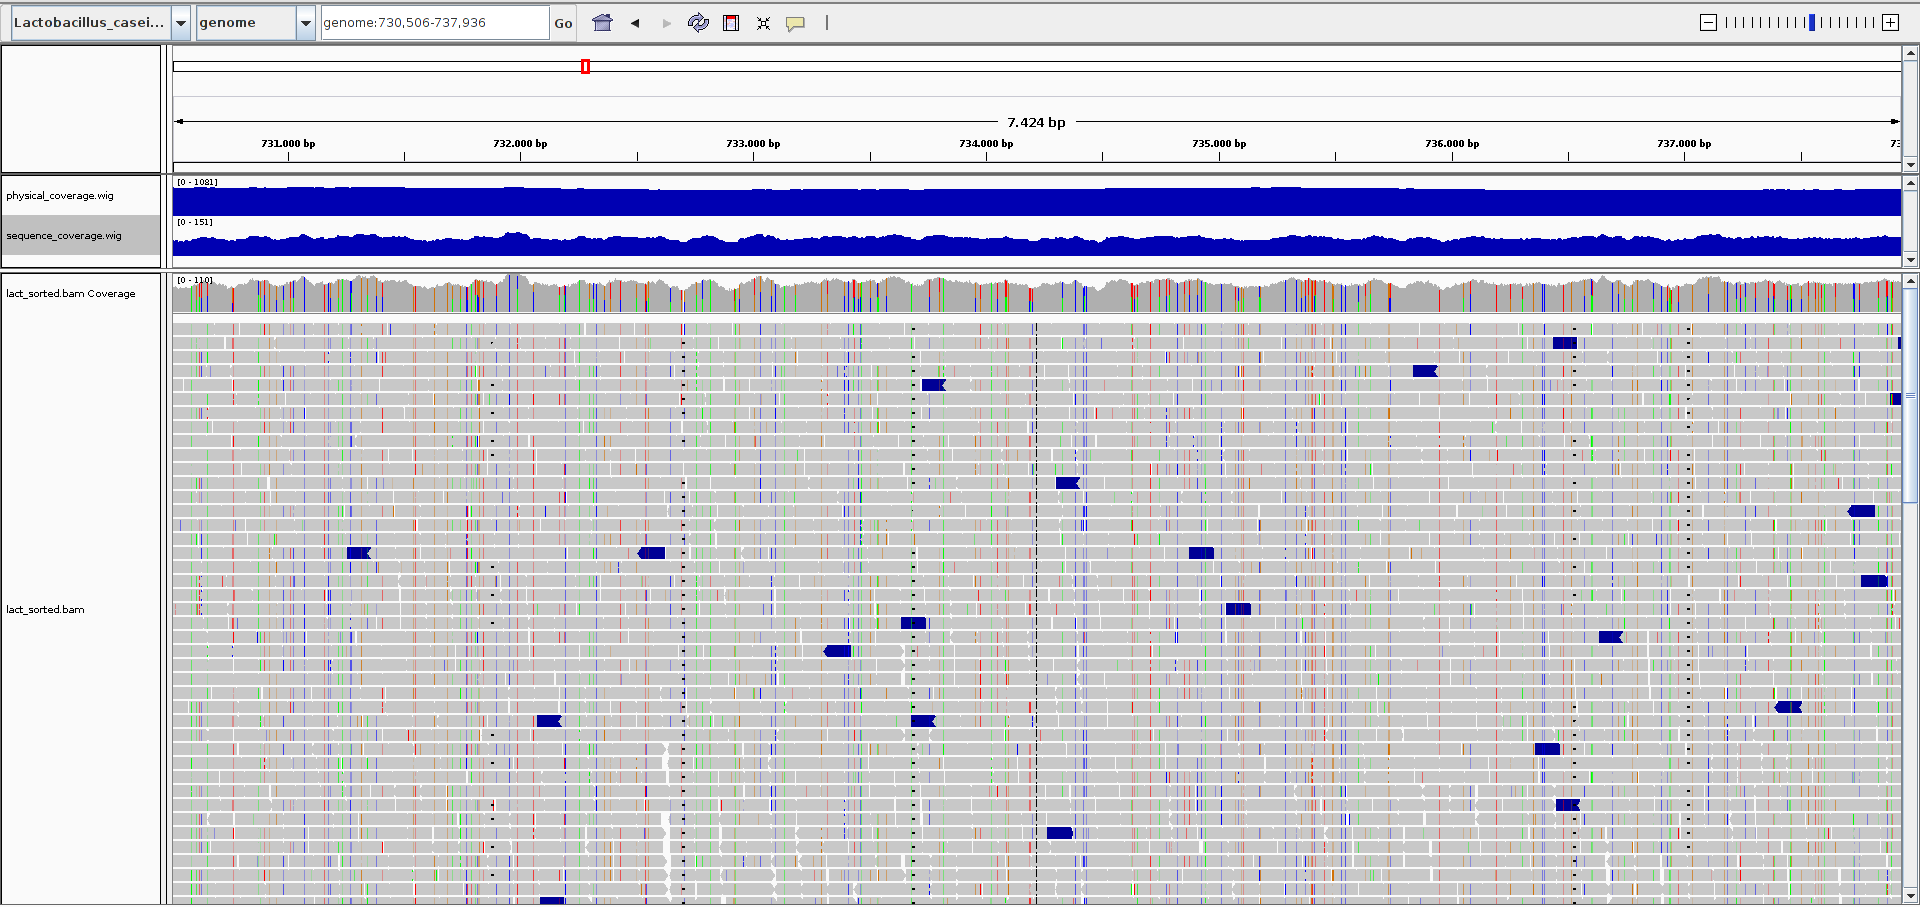
\includegraphics[scale=0.2]{img/pairs2}
  \caption{Some insertions}
  \label{fig:pairs2}
\end{figure}

\end{enumerate}

\newpage
\subsection{Part 2}

\begin{enumerate}
\setcounter{enumi}{8}
  \item Implement in the language of your choice a program to create a wig
file with physical covarage.
An example can be found in physical.pl, but it would be nice to implement
the suggestions described in physical\_coverage.pdf
  \item Create a wig track with sequence coverage and compare it with the
IGV track
  \item Read the sam file and for each mate pair calculate the length of the
genomic insert; then calculate the mean and standard deviation of the inserts,
possibly discarding those that are totally out of range
A plot of the length distribution may help to evaluate the sizes
  \item Create a track with the percentage of inserts with a length exceeding
n standard deviations (for instance n=2) above or below the mean
  \item Comment the results
\end{enumerate}

\subsection{Part 2 - Answers}

\begin{enumerate}
\setcounter{enumi}{8}
  \item Python script for physical coverage, given the sam file and
length of the reference genome:
\lstinputlisting[language=Python]{scripts/physical.py}
  \item Python script for sequence coverage, given the sam file and
length of the reference genome:
\lstinputlisting[language=Python]{scripts/sequence.py}
The wig track for sequence coverage generated is almost similar to the IGV
track.
So far the tracks created are the physical coverage and the genetic coverage:

\begin{figure}[h]
  \centering
  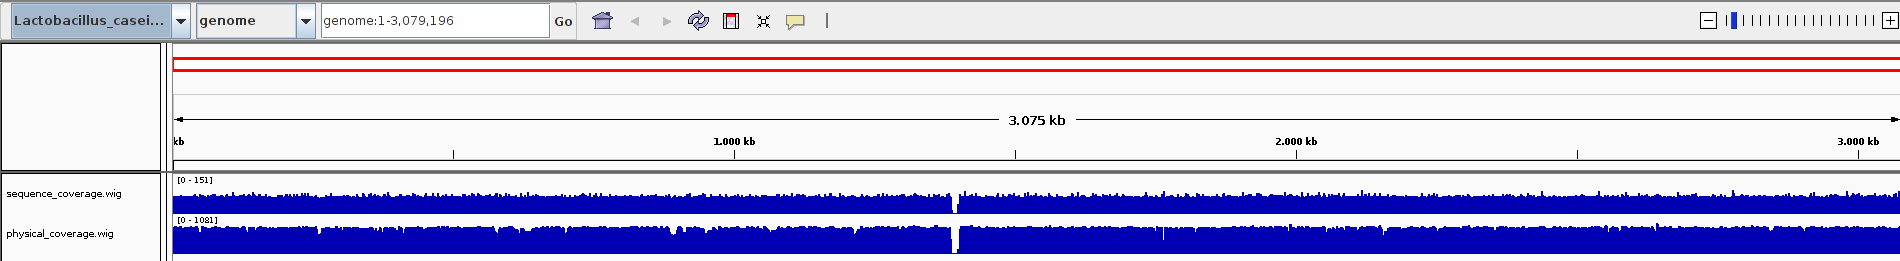
\includegraphics[scale=0.2]{img/ps_tracks}
  \caption{Physical and genetic coverage}
\end{figure}

  \item Python script to calculate the insert length, given the sam file and
length of the reference genome:
\lstinputlisting[language=Python]{scripts/insert.py}

In the previous calculation I suppose that the two reads for a mate pair have
the same length.

Python script to calculate the mean and the standard deviation, given the
wiggle file with the insert lengths:
\lstinputlisting[language=Python]{scripts/insert_mean_sd.py}

The mean is: \textbf{2220} \\

The standard deviation has been calculated by the formula: 

\begin{equation}
SD = \sqrt{\frac{\Sigma|x-\bar{x}|^2}{n}}
\end{equation}

and its value is: $\sigma = \textbf{203.495}$ without discarding any value.

  \item Python script to calculate the inserts above or below the standard
deviation by thrice \textbf{(n = 3)}, given the wiggle file with the insert
lengths:
\lstinputlisting[language=Python]{scripts/deviations.py}

In figure \ref{img:plot} we can see that some insert are longer than 12000 bases.
The longest insert is 16281 bases long.

\begin{figure}[h]
  \centering
  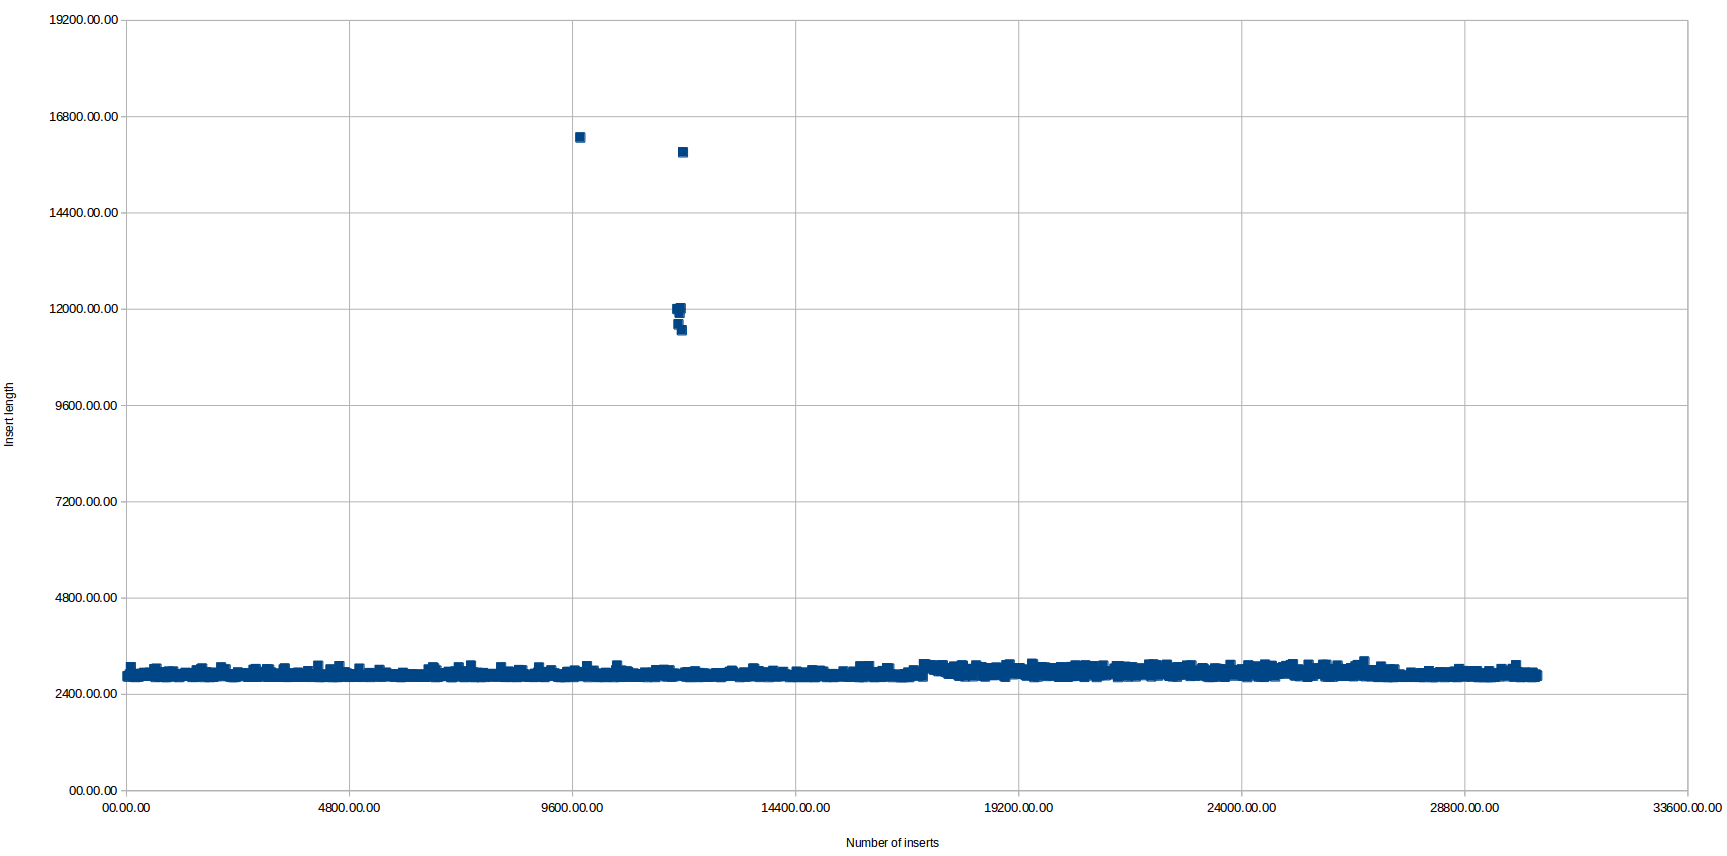
\includegraphics[scale=0.2]{img/plot}
  \caption{Plot for length of inserts}
  \label{img:plot}
\end{figure}

\end{enumerate}
